%%%%%%%%%%%%%%%%%%%%%%%%%%%%%%%%%%%%%%%%%
% Awesome Resume/CV
% XeLaTeX Template
% Version 1.2 (27/3/2017)
%
% This template has been downloaded from:
% http://www.LaTeXTemplates.com
%
% Original author:
% Claud D. Park (posquit0.bj@gmail.com) with modifications by 
% Vel (vel@latextemplates.com)
%
% License:
% CC BY-NC-SA 3.0 (http://creativecommons.org/licenses/by-nc-sa/3.0/)
%
% Important note:
% This template must be compiled with XeLaTeX, the below lines will ensure this
%!TEX TS-program = xelatex
%!TEX encoding = UTF-8 Unicode
%
%%%%%%%%%%%%%%%%%%%%%%%%%%%%%%%%%%%%%%%%%

%----------------------------------------------------------------------------------------
%	PACKAGES AND OTHER DOCUMENT CONFIGURATIONS
%----------------------------------------------------------------------------------------

\documentclass[11pt, a4paper]{awesome-cv} % A4 paper size by default, use 'letterpaper' for US letter
\usepackage{natbib}
%\usepackage{bibentry}
\usepackage{enumerate}
\bibliographystyle{abbrvnat} % or plainnat or plain or acm or apalike or ...
\bibpunct{(}{)}{;}{a}{}{,} % see http://merkel.zoneo.net/Latex/natbib.php

\usepackage{bibentry} % place bibliographic entries anywhere in the text

\geometry{left=2cm, top=1.5cm, right=2cm, bottom=2cm, footskip=.5cm} % Configure page margins with geometry

\fontdir[fonts/] % Specify the location of the included fonts

% Color for highlights
\colorlet{awesome}{awesome-red} % Default colors include: awesome-emerald, awesome-skyblue, awesome-red, awesome-pink, awesome-orange, awesome-nephritis, awesome-concrete, awesome-darknight
%\definecolor{awesome}{HTML}{CA63A8} % Uncomment if you would like to specify your own color

% Colors for text - uncomment and modify
%\definecolor{darktext}{HTML}{414141}
%\definecolor{text}{HTML}{414141}
%\definecolor{graytext}{HTML}{414141}
%\definecolor{lighttext}{HTML}{414141}

\renewcommand{\acvHeaderSocialSep}{\quad\textbar\quad} % If you would like to change the social information separator from a pipe (|) to something else

%----------------------------------------------------------------------------------------
%	PERSONAL INFORMATION
%	Comment any of the lines below if they are not required
%----------------------------------------------------------------------------------------

\name{Van Cam}{PHAM}
\address{2, Jacques Margottin, Bourg-la-reine, 92340, France}
\mobile{(+33) 07 50 89 72 11}

\email{phamvancam2104@gmail.com, vancam.pham@cea.fr}
%\email{vancam.pham@cea.fr}
%\homepage{www.posquit0.com}
%\github{posquit0}
%\linkedin{posquit0}
%\skype{skypeid}
%\stackoverflow{SOid}{SOname}
%\twitter{@twit}
%\linkedin{linkedin name}
%\reddit{reddit account}
%\xing{xing name}
%\extrainfo{test} % Other text you want to include on this line

\position{Software Engineer/PhD in Model-Based Software Engineering (11/2014-1/2018[anticipated])} % Your expertise/fields
%\quote{``Make the change that you want to see in the world."} % A quote or statement

\makecvfooter{\today}{Văn Cam. PHẠM~~~·~~~Résumé}{\thepage} % Specify the letter footer with 3 arguments: (<left>, <center>, <right>), leave any of these blank if they are not needed

%----------------------------------------------------------------------------------------

\begin{document}

\makecvheader % Print the header 
\hfill \begin{picture}(0,20)
\put(400,0){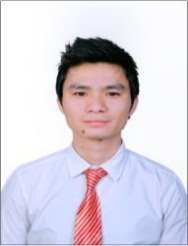
\includegraphics[width=7.5em]{photoCam.jpg}}
\end{picture}

%----------------------------------------------------------------------------------------
%	CV/RESUME CONTENT
%	Each section is imported separately, open each file in turn to modify content
%----------------------------------------------------------------------------------------

%----------------------------------------------------------------------------------------
%	SECTION TITLE
%----------------------------------------------------------------------------------------

\cvsection{Education}

%----------------------------------------------------------------------------------------
%	SECTION CONTENT
%----------------------------------------------------------------------------------------

\begin{cventries}

%------------------------------------------------

\cventry
{Thesis Title: Methothodologies for model-code synchronization for reactive system development} % Degree
{Software Engineer/PhD at LISE (Laboratory of Model-Driven Engineering for Embedded Systems)} % Institution
{Saclay, France} % Location
{Nov. 2014 - Nov. 2017 [anticipated]} % Date(s)
{ % Description(s) bullet points
	\begin{cvitems}
		\item {\textbf{Working place}: Laboratory of Model-Driven Engineering for Embedded Systems (LISE), CEA-List, Saclay, France.}	
		\item {\textbf{Brief Synopsis}: I worked as a software engineer as well as a PhD candidate in the Laboratoire d'Ingénierie dirigée par les modèles pour les systèmes embarqués in the domain design and implementation of reactive application in the context of Model-Based Software Engineering (MBSE) and component-based architecture design. 
		MBSE focuses on using abstract diagram-based modeling languages such as UML to design complex and distributed system architecture. 
		I develop a framework, which allows to (1) use UML to design complex system software and automatically generate C/C++ code of the high-level application behavior; (2) develop algorithmic/computational code for applications; and (3) propagate the modifications in code back to the UML design to update the design and to keep it consistent with the code. 
		Code productivity is significantly gained by the ability to automatically produce code from design. Furthermore, C/C++ code is efficient and many bugs in code are eliminated because of the use of automatic code generation. That is to say that, the approach benefits advantages of both of MBSE such as complexity management, productivity  and communication by UML, and traditional software programming, which is one of the most important tasks during software development with many strong and widely used programming languages such as Java and C++.  
		%My thesis is to propose an approach for combining both of the modeling and programming practice to benefit their advantages. 
		%Specifically, I propose a synchronization approach, which keeps UML-based software architecture model and object-oriented programming code such as C++ and Java consistent in case there are modifications of the model and the code. 
		%The software structure is designed based on component-based engineering, which enables decoupling between software components and re-usability of components. 
		%The software behavior is described by using state machines, which are appropriate to manage the discrete event-driven reactive system behaviors.
	} 
	\end{cvitems}
}

\cventry
{Master in Embedded Systems and Signal Processing} % Degree
{U-PSUD(University of Paris-Sud)} % Institution
{Orsay, France} % Location
{Sept. 2013 - Sept. 2014} % Date(s)
{ % Description(s) bullet points
	\begin{cvitems}
		\item {Program: Embedded Systems and Signal Processing (SETI) cooperated by University of Paris Sud, ENS Cachan, INSTN and ENSTA ParisTech, France}		
		\item {Scholarship Student of International Relationships of University of Paris-Sud}
		\item {Modules included: Real-time Control Numeric Systems, Complex Embedded System Design, Algorithm-Architecture Ad-equation, Network and Quality of Services, Multimedia Data Compression, Data Fusion, Statistic Learning and Neural Network, and Initiation to Research.}
	\end{cvitems}
}


\cventry
{Engineer in Information System and Communication} % Degree
{HUST(Hanoi University of Science and Technology)} % Institution
{Hanoi, Vietnam} % Location
{Sept. 2007 - Jul. 2012} % Date(s)
{ % Description(s) bullet points
\begin{cvitems}
\item {Program: Programme de Formation d'Ingenieur d'Excellence au Vietnam (PFIEV) - Programming of Training for Excellent Engineers in Vietnam}
\item {Final project: Understanding pros and cons of the client-server and peer-to-peer models, and combining these two models for developing distributed applications.}
\end{cvitems}
}

%------------------------------------------------

\end{cventries}
%\vspace{1cm}
\cvsection{Employment}

\begin{cventries}

\cventry
{Software Engineer/PhD Student at Laboratory of Model-Driven Engineering for Embedded Systems (LISE)} % Degree
{Laboratory of Model-Driven Engineering for Embedded Systems (LISE), CEA-LIST} % Institution
{CEA, Saclay, France} % Location
{Nov. 2014 - Jan. 2018} % Date(s)
{ % Description(s) bullet points
	\begin{cvitems}
		\item {I have been working as a software engineering and PhD Student, under supervision of Dr. Ansgar RADERMACHER, Dr. S\'ebastien G\'ERARD, and Dr. Shuai LI, at LISE, which develops the Papyrus industrial modeling tool, especially the use of UML to design complex system software. My work involves: the use of UML for designing component-based architecture and event-driven behaviors for reactive and distributed systems in the context of the Papyrus Designer tool; the corresponding implementation of the UML-based design; the process of automatically translating the UML-based software design model into efficient executable code; and the process of automatically propagating modifications of the code back to the model. Technically, I have been working with several mainstream programming languages such as Java, C++, and C and have a deep understanding of the programming languages in order to generate code from models. I also extend the standard C++ programming language to support component-based developemnt for better managing complexity in code-centric development approaches, especially for reactive systems. An Arm-based Lego Car factory application is developed for demonstration.}		
	\end{cvitems}
}


\cventry
{Internship at Laboratory of Model-Driven Engineering for Embedded Systems (LISE)} % Degree
{Laboratory of Model-Driven Engineering for Embedded Systems (LISE), CEA-LIST} % Institution
{CEA, Saclay, France} % Location
{Apr. 2014 - Sept. 2014} % Date(s)
{ % Description(s) bullet points
	\begin{cvitems}
		\item {I worked as an intern undersupervison of Dr. Ansgar RADERMACHER in the context of applying component-based modeling and design to distributed system development. I used UML and a UML profile for designing interactions between distributed components in distributed systems. The created design is then automatically translated into code, which uses the ZeroMQ middleware to exchange data between distributed components.}		
	\end{cvitems}
}


\cventry
{Software Engineer for Computers and Embedded System} % Degree
{Toshiba Software Development Vietnam (TSDV)} % Institution
{Hanoi, Vietnam} % Location
{Jul. 2012 - Aug. 2013} % Date(s)
{ % Description(s) bullet points
	\begin{cvitems}
		\item {I worked as a software developer in three projects: (1) deal with requirement analysis, detailed design, implementation, unit test, integration test, and optimization at the programming level for software of an embedded system: Toshiba G2R protection relay. The development using C as the development language and Visual Studio as an integrated development environment (IDE) includes using IEC 60870-5-103 to control and communicate between smart electric device, and testing on real hardware and using debug tools to debug on hardware; (2) develop a desktop application to control electric devices by using a private protocol of Toshiba and the C\# language. The application polls the devices to receive data of recorded errors, and creates a chart for analysis of errors causes; and (3) use the Qt IDE and the C++ ffmpeg library for implementing a multimedia player application, which plays both audio and video files.}		
	\end{cvitems}
}

%\cventry
{Internship for developing games and applications for Android} % Degree
{Tamtay.vn Company} % Institution
{Hanoi, Vietnam} % Location
{Feb. 2012 - Apr. 2012} % Date(s)
{ % Description(s) bullet points
	\begin{cvitems}
		\item {I worked as an intern at the tamtay.vn company, that develops applications and games for the tamtay.vn social network. My responsibility is to investigate the development framework Android SDK for Android applications. I then collaborated with another intern to develop a simple multimedia player application, that downloads and plays music files and associated information transfered in JSON files. I was then responsible for investigating the AndEngine game engine to learn skills in game development.}		
	\end{cvitems}
}

\cventry
{Internship for investigating Google Cloud Platform} % Degree
{School of Communication and Information Technology - Hanoi University of Science and Technology} % Institution
{Hanoi, Vietnam} % Location
{Jul. 2011 - Aug. 2011} % Date(s)
{ % Description(s) bullet points
	\begin{cvitems}
		\item {I worked as an intern at the School of Communication and Information Technology. I investigated the \textit{Google App Engine} Google Cloud Platform for building scalable webs and mobile backends using Java, Eclipse IDE, TomCat, plugin of Google App Engine for Java.}		
	\end{cvitems}
}

\end{cventries}

%\newpage % Force a new page for looks
%-------------------------------------------------------------------------------
%	SECTION TITLE
%-------------------------------------------------------------------------------
\cvsection{Skills}


%-------------------------------------------------------------------------------
%	CONTENT
%-------------------------------------------------------------------------------
\begin{cvskills}

%---------------------------------------------------------
  \cvskill
    {Programming} % Category
    {Python, Node.JS, C/C++, Scala, JAVA, OCaml, LaTeX} % Skills

%---------------------------------------------------------
  \cvskill
    {Web} % Category
    {Django, Express, Redux, React, HTML5, LESS, SASS} % Skills

%---------------------------------------------------------
  \cvskill
    {Languages} % Category
    {Korean, English, Japanese, Chinese} % Skills

%---------------------------------------------------------
\end{cvskills}

%%----------------------------------------------------------------------------------------
%	SECTION TITLE
%----------------------------------------------------------------------------------------

\cvsection{Experience}

%----------------------------------------------------------------------------------------
%	SECTION CONTENT
%----------------------------------------------------------------------------------------

\begin{cventries}

%------------------------------------------------

\cventry
{Software Engineer \& Security Researcher (Compulsory Military Service)} % Job title
{R.O.K Cyber Command, MND} % Organization
{Seoul, S.Korea} % Location
{Aug. 2014 - Exp. Apr. 2016} % Date(s)
{ % Description(s) of tasks/responsibilities
\begin{cvitems}
\item {Implemented a military cooperation system which is web based real time messenger in Scala on Lift.}
\item {Improved functionality on military command and control system for incident response with Java Servlet.}
\item {Lead engineer on agent-less backtracking system that can discover client device's fingerprint(including public and private IP) independently of the Proxy, VPN and NAT.}
\end{cvitems}
}

%------------------------------------------------    

\cventry
{Game Developer Intern at Global Internship Program} % Job title
{NEXON} % Organization
{Seoul, S.Korea \& LA, U.S.A} % Location
{Jan. 2013 - Feb. 2013} % Date(s)
{ % Description(s) of tasks/responsibilities
\begin{cvitems}
\item {Developed in Cocos2d-x an action puzzle game(Dragon Buster) targeting U.S. market. Implemented API server which is communicating with game client and In-App Store, along with two other team members who wrote the game logic, designed game graphics.}
\item {Won the 2nd prize in final evaluation.}
\end{cvitems}
}

%------------------------------------------------

\cventry
{Researcher for <Detecting video’s torrents using image similarity algorithms>} % Job title
{Undergraduate Research, Computer Vision Lab(Prof. Bohyung Han)} % Organization
{Pohang, S.Korea} % Location
{Sep. 2012 - Feb. 2013} % Date(s)
{ % Description(s) of tasks/responsibilities
\begin{cvitems}
\item {Researched means of retrieving a corresponding video based on image contents using image similarity algorithm.}
\item {Implemented prototype that users can obtain torrent magnet links of corresponding video relevant to an image on web site.}
\end{cvitems} 
}

%------------------------------------------------

\cventry
{Software Engineer Trainee} % Job title
{Software Maestro (funded by Korea Ministry of Knowledge and Economy)} % Organization
{Seoul, S.Korea} % Location
{Jul. 2012 - Jun. 2013} % Date(s)
{ % Description(s) of tasks/responsibilities
\begin{cvitems}
\item {Performed research memory management strategies of OS and implemented in Python an interactive simulator for Linux kernel memory management.}
\end{cvitems}
}

%------------------------------------------------

\cventry
{Software Engineer} % Job title
{ShitOne Corp. (Start-up company)} % Organization
{Seoul, S.Korea} % Location
{Dec. 2011 - Feb. 2012} % Date(s)
{ % Description(s) of tasks/responsibilities
\begin{cvitems}
\item {Developed a proxy drive smartphone application which connects proxy driver and customer. Implemented overall Android application logic and wrote API server for community service, along with lead engineer who designed bidding protocol on raw socket and implemented API server for bidding.}
\end{cvitems}
}

%------------------------------------------------

\cventry
{Freelance Penetration Tester} % Job title
{SAMSUNG Electronics} % Organization
{S.Korea} % Location
{Sep. 2013, Mar. 2011 - Oct. 2011} % Date(s)
{ % Description(s) of tasks/responsibilities
\begin{cvitems}
\item {Conducted penetration testing on SAMSUNG KNOX, which is solution for enterprise mobile security.}
\item {Conducted penetration testing on SAMSUNG Smart TV.}
\end{cvitems}
}

%------------------------------------------------

\end{cventries}
%\vspace{1cm}
\newpage
\cvsection{Topics of Interests}
\begin{cventries}

\cvinterest
{Software programming language, software architecture design and implementation}
{
	\begin{cvitems}
		\item{As a PhD student and a practitioner in software engineering, I am passionate in programming, especially the use of mainstream programming languages such as C/C++, Java, and Python for development of software applications (e.g. reactive embedded system applications) for solving everyday life problems. I'm also interested in knowing practices how to be productive and qualitative in programming.}
		\item{A major part of my thesis work is about extending, engineering, and transforming software programming language. Especially, I'm interested in extending current programming languages to assist developers to be productive and qualitative in software development.}
		\item{During PhD time, I have learned about application of event-driven architecture to asynchronous systems such as distributed systems. I'm interested in using programming model and network protocols to develop distributed and/or embedded applications, which will involve network technologies such as communication protocols or routing algorithms as well as the combination of peer-to-peer and client-server model as in my undergraduate at HUST.}
	\end{cvitems}
}


\cvinterest
{Research and Development of Embedded and Distributed Systems}
{\begin{cvitems}
		\item{In my thesis, I work in the context of development of embedded software systems, in which I use UML and design patterns for designing such systems (or software in general). I'm therefore interested in diving into this domain as deep as possible. Furthermore, I want to combine my knowledge about the network technologies that I have collected to produce distributed embedded software systems. The latter, in my thought, are very suitable to the development (design and coding) of IoT applications, in which devices collect, process, and exchange data with each other, and which might be combined with machine learning field. Using UML, from my point of view, would be very helpful for the complexity management task of such systems.}
\end{cvitems}}

\cvinterest
{Machine learning}
{\begin{cvitems}
		\item{The field of machine learning and its application have been attracting many practitioners including myself.
During my master education, I was taught about machine learning (modules data fusion and statistic learning and neural network). 
Since there, I have been keeping my passion and learning practically, especially using Python, the use of different learning models for understanding data and prediction.}
\end{cvitems}
}

\cvinterest
{Model-Based Software Engineering}
{
	\begin{cvitems}
	\item{The main research interest of my PhD thesis are methodologies for synchronization of code and model specified in UML-based component-based modeling and UML state machines, and studying different techniques for model transformation such as QVT, ATL, Triple-Graph Grammar (TGG), and Change-driven transformation, for model synchronization such as QVT-Relation and TGG.	
I'm also involved in researching approaches for a mapping of a UML model containing the ALF code, and programming language code.
This mapping will enable a synchronization of UML model with ALF and programming code, and eventually provide synchronization of a platform-independent model with code.
Furthermore, I'm also interested in approaches for simulating a system from its models and generating fully operational code from models, especially UML models, which might contain ALF code, approaches for optimizing software system at the model level (e.g. optimization ALF code or UML state machines), and if possibly approaches for model interpretation and compilation.
The final goal is harmonization of software programming and MDE practices.}
\end{cvitems}}


\cvinterest
{Leisure}
{Football watching, tourism, book reading (especially historical + technical books, or sometimes literature), chatting}

\begin{comment}
\cvinterest
{Model-Driven Engineering with Large Models}
{
	\begin{cvitems}
		\item {I have been working with Papyrus UML models during my thesis for generating real case-study embedded systems, e.g. 12000 lines of code generated for the Lego Car factory case study. When models become large, the processing of the models, e.g. querying and loading for model transformations, becomes very slow, which might harms the adoption of modeling techniques to industrial development. For this, I'm very interested in studying techniques for speeding model manipulations up such as incremental model query with IncQuery or the PrefetchML prefetching and caching language for caching models.}
	\end{cvitems}
}
\end{comment}


\end{cventries}


%\vspace{1cm}
\cvsection{References}
\begin{table}[h]
	\centering
	\descriptionstyle{\begin{tabular}{p{0.32\textwidth}p{0.32\textwidth}p{0.32\textwidth}}
		Dr. Ansgar RADERMACHER        & Dr. Shuai LI                  & Dr. Sebastien GERARD          \\
		Ansgar.RADERMACHER@cea.fr     & Shuai.LI@cea.fr               & Sebastien.GERARD@cea.fr       \\
		Laboratory: LISE              & Laboratory: LISE              & Laboratory: LISE- Papyrus development              \\
		CEA-LIST, CEA, Saclay, France & CEA-LIST, CEA, Saclay, France & CEA-LIST, CEA, Saclay, France
	\end{tabular}}
\end{table}




%-------------------------------------------------------------------------------
%	SECTION TITLE
%-------------------------------------------------------------------------------
\cvsection{Publications}
\renewcommand\refname{Conference Proceedings and Journal Articles}
%-------------------------------------------------------------------------------
%	SUBSECTION TITLE
%-------------------------------------------------------------------------------
%\cvsubsection{Conference Proceedings and Journal Articles}
\descriptionstyle{
%\nobibliography*
%\bibliographystyle{plain}	
\bibliography{refs}
\begin{itemize}
	%\item \bibentry{completeusmspringer}	\item \bibentry{DBLP:conf/icsa/PhamRGL17}	\item \bibentry{DBLP:conf/modelsward/PhamRGL17}	\item \bibentry{DBLP:conf/iceccs/PhamLRGM16}	\item \bibentry{DBLP:conf/fedcsis/PhamRG16}	\item \bibentry{DBLP:conf/modelsward/PhamRGN16}	\item \bibentry{Pham2014}
\end{itemize}
}


%s\vspace{1cm}
%-------------------------------------------------------------------------------
%	SECTION TITLE
%-------------------------------------------------------------------------------
\cvsection{Presentation}


%-------------------------------------------------------------------------------
%	CONTENT
%-------------------------------------------------------------------------------
\begin{cventries}

%---------------------------------------------------------
  \cventry
    {Presenter for <DEFCON 20th : The way to go to Las Vegas>} % Role
    {6th CodeEngn (Reverse Engineering Conference)} % Event
    {Seoul, S.Korea} % Location
    {Jul. 2012} % Date(s)
    {
      \begin{cvitems} % Description(s)
        \item {Introduced CTF(Capture the Flag) hacking competition and advanced techniques and strategy for CTF}
      \end{cvitems}
    }

%---------------------------------------------------------
  \cventry
    {Presenter for <Metasploit 101>} % Role
    {6th Hacking Camp - S.Korea} % Event
    {S.Korea} % Location
    {Sep. 2012} % Date(s)
    {
      \begin{cvitems} % Description(s)
        \item {Introduced basic procedure for penetration testing and how to use Metasploit}
      \end{cvitems}
    }

%---------------------------------------------------------
\end{cventries}

%%-------------------------------------------------------------------------------
%	SECTION TITLE
%-------------------------------------------------------------------------------
\cvsection{Honors \& Awards}


%-------------------------------------------------------------------------------
%	SUBSECTION TITLE
%-------------------------------------------------------------------------------
\cvsubsection{International}


%-------------------------------------------------------------------------------
%	CONTENT
%-------------------------------------------------------------------------------
\begin{cvhonors}

%---------------------------------------------------------
  \cvhonor
    {Finalist} % Award
    {DEFCON 22nd CTF Hacking Competition World Final} % Event
    {Las Vegas, U.S.A} % Location
    {2014} % Date(s)

%---------------------------------------------------------
  \cvhonor
    {Finalist} % Award
    {DEFCON 21st CTF Hacking Competition World Final} % Event
    {Las Vegas, U.S.A} % Location
    {2013} % Date(s)

%---------------------------------------------------------
  \cvhonor
    {Finalist} % Award
    {DEFCON 19th CTF Hacking Competition World Final} % Event
    {Las Vegas, U.S.A} % Location
    {2011} % Date(s)

%---------------------------------------------------------
  \cvhonor
    {6th Place} % Award
    {SECUINSIDE Hacking Competition World Final} % Event
    {Seoul, S.Korea} % Location
    {2012} % Date(s)

%---------------------------------------------------------
\end{cvhonors}


%-------------------------------------------------------------------------------
%	SUBSECTION TITLE
%-------------------------------------------------------------------------------
\cvsubsection{Domestic}


%-------------------------------------------------------------------------------
%	CONTENT
%-------------------------------------------------------------------------------
\begin{cvhonors}

%---------------------------------------------------------
  \cvhonor
    {3rd Place} % Award
    {WITHCON Hacking Competition Final} % Event
    {Seoul, S.Korea} % Location
    {2015} % Date(s)

%---------------------------------------------------------
  \cvhonor
    {Silver Prize} % Award
    {KISA HDCON Hacking Competition Final} % Event
    {Seoul, S.Korea} % Location
    {2013} % Date(s)

%---------------------------------------------------------
  \cvhonor
    {2nd Award} % Award
    {HUST Hacking Festival} % Event
    {S.Korea} % Location
    {2013} % Date(s)

%---------------------------------------------------------
  \cvhonor
    {3rd Award} % Award
    {HUST Hacking Festival} % Event
    {S.Korea} % Location
    {2010} % Date(s)

%---------------------------------------------------------
  \cvhonor
    {3rd Award} % Award
    {Holyshield 3rd Hacking Festival} % Event
    {S.Korea} % Location
    {2012} % Date(s)

%---------------------------------------------------------
  \cvhonor
    {2nd Award} % Award
    {Holyshield 3rd Hacking Festival} % Event
    {S.Korea} % Location
    {2011} % Date(s)

%---------------------------------------------------------
  \cvhonor
    {5th Place} % Award
    {PADOCON Hacking Competition Final} % Event
    {Seoul, S.Korea} % Location
    {2011} % Date(s)

%---------------------------------------------------------
\end{cvhonors}



%%-------------------------------------------------------------------------------
%	SECTION TITLE
%-------------------------------------------------------------------------------
\cvsection{Extracurricular Activity}


%-------------------------------------------------------------------------------
%	CONTENT
%-------------------------------------------------------------------------------
\begin{cventries}

%---------------------------------------------------------
  \cventry
    {Core Member \& President at 2013} % Affiliation/role
    {PoApper (Developers' Network of POSTECH)} % Organization/group
    {Pohang, S.Korea} % Location
    {Jun. 2010 - PRESENT} % Date(s)
    {
      \begin{cvitems} % Description(s) of experience/contributions/knowledge
        \item {Reformed the society focusing on software engineering and building network on and off campus.}
        \item {Proposed various marketing and network activities to raise awareness.}
      \end{cvitems}
    }

%---------------------------------------------------------
  \cventry
    {Member} % Affiliation/role
    {PLUS (Laboratory for UNIX Security in POSTECH)} % Organization/group
    {Pohang, S.Korea} % Location
    {Sep. 2010 - Oct. 2011} % Date(s)
    {
      \begin{cvitems} % Description(s) of experience/contributions/knowledge
        \item {Gained expertise in hacking \& security areas, especially about internal of operating system based on UNIX and several exploit techniques.}
        \item {Participated on several hacking competition and won a good award.}
        \item {Conducted periodic security checks on overall IT system as a member of POSTECH CERT.}
        \item {Conducted penetration testing commissioned by national agency and corporation.}
      \end{cvitems}
    }

%---------------------------------------------------------
\end{cventries}


%%----------------------------------------------------------------------------------------
%	SECTION TITLE
%----------------------------------------------------------------------------------------

\cvsection{Writing}

%----------------------------------------------------------------------------------------
%	SECTION CONTENT
%----------------------------------------------------------------------------------------

\begin{cventries}

%------------------------------------------------

\cventry
{Founder \& Writer} % Role
{A Guide for Developers in Start-up} % Title
{Facebook Page} % Location
{Jan. 2015 - PRESENT} % Date(s)
{ % Description(s)
\begin{cvitems}
\item {Drafted daily news for developers in Korea about IT technologies, issues about start-up.}
\end{cvitems}
}

%------------------------------------------------

\cventry
{Undergraduate Student Reporter} % Role
{AhnLab} % Title
{S.Korea} % Location
{Oct. 2012 - Jul. 2013} % Date(s)
{ % Description(s)
\begin{cvitems}
\item {Drafted reports about IT trends and Security issues on AhnLab Company magazine.}
\end{cvitems}
}

%------------------------------------------------

\end{cventries}
%%-------------------------------------------------------------------------------
%	SECTION TITLE
%-------------------------------------------------------------------------------
\cvsection{Program Committees}


%-------------------------------------------------------------------------------
%	CONTENT
%-------------------------------------------------------------------------------
\begin{cvhonors}

%---------------------------------------------------------
  \cvhonor
    {Problem Writer} % Position
    {2016 CODEGATE Hacking Competition World Final} % Committee
    {S.Korea} % Location
    {2016} % Date(s)

%---------------------------------------------------------
  \cvhonor
    {Organizer \& Co-director} % Position
    {1st POSTECH Hackathon} % Committee
    {S.Korea} % Location
    {2013} % Date(s)

%---------------------------------------------------------
  \cvhonor
    {Staff} % Position
    {7th Hacking Camp} % Committee
    {S.Korea} % Location
    {2012} % Date(s)

%---------------------------------------------------------
  \cvhonor
    {Problem Writer} % Position
    {1st Hoseo University Teenager Hacking Competition} % Committee
    {S.Korea} % Location
    {2012} % Date(s)

%---------------------------------------------------------
  \cvhonor
    {Staff \& Problem Writer} % Position
    {JFF(Just for Fun) Hacking Competition} % Committee
    {S.Korea} % Location
    {2012} % Date(s)

%---------------------------------------------------------
\end{cvhonors}


%----------------------------------------------------------------------------------------

\end{document}